%!TEX root = main.tex
Consider the following mini convolutional neural net, where $(x_1, x_2, x_3)$ is the input,
followed by a convolution layer with a filter $(w_1, w_2)$, a ReLU layer, and a fully connected layer with weight $(v_1, v_2)$.

 

\tikzstyle{vertex}=[circle,draw=black,minimum size=20pt,inner sep=0pt]
\tikzstyle{edge} = [draw,thick,-]
%\tikzstyle{emptyvertex}=[circle,draw=white,minimum size=10pt,inner sep=0pt]
\tikzstyle{weight} = [font=\small]

\begin{center}
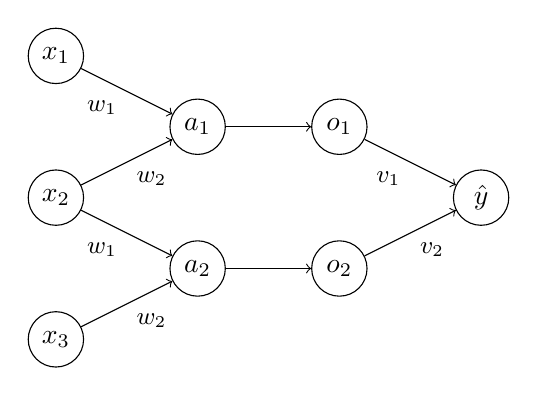
\begin{tikzpicture}[scale=.9, auto,swap]
\foreach \pos/\name in { {(0,5)/x_1}, {(0, 3)/x_2}, {(0, 1)/x_3},  {(2, 4)/a_1}, {(2, 2)/a_2},  {(4, 4)/o_1}, {(4, 2)/o_2}}
\node[vertex] (\name) at \pos {$\name$};
\node[vertex] (y) at (6, 3) {$\hat{y}$};
\foreach \source/ \dest /\weight in {x_1/a_1/w_1, x_2/a_1/w_2, x_2/a_2/w_1, x_3/a_2/w_2, a_1/o_1/, a_2/o_2/, o_1/y/v_1, o_2/y/v_2}
\draw[->] (\source) edge node[weight] {$\weight$} (\dest);
\end{tikzpicture}
\end{center}

 

More concretely, the computation is specified by
\begin{align*}
a_1 &= x_1 w_1 + x_2 w_2 \\
a_2 &= x_2 w_1 + x_3 w_2 \\
o_1 &= \max\{0, a_1\} \\
o_2 &= \max\{0, a_2\} \\
\hat{y} &= o_1 v_1 + o_2 v_2 
\end{align*}

For an example $(\vx, y) \in \R^3 \times \{-1, +1\}$,  the logistic loss of the CNN is
\[
\ell = \ln(1 + \exp(-y\hat{y})),
\]
which is a function of the parameters of the network: $w_1, w_2, v_1, v_2$.\\


\textbf{2.1} (\blue{4pts})
Write down $\frac{\partial \ell}{\partial v_1}$  and $\frac{\partial \ell}{\partial v_2}$ (show the intermediate steps that use chain rule).
You can use the sigmoid function $\sigma(z) = \frac{1}{1+e^{-z}}$ to simplify your notation.\\

\noindent{\fontsize{11}{12}\selectfont\textbf{Solution 2.1}}

\[
\ell = \ln(1+\exp(-y\hat y)),
\qquad
\hat y = o_1v_1 + o_2v_2.
\]

First, compute the derivative of the loss with respect to $\hat y$:
\begin{align*}
\frac{\partial \ell}{\partial \hat y}
&= \frac{1}{1+\exp(-y\hat y)} \cdot \exp(-y\hat y)\cdot (-y) \\
&= -y \frac{\exp(-y\hat y)}{1+\exp(-y\hat y)} \\
&= -y\,\sigma(-y\hat y),
\end{align*}
where $\sigma(z)=\frac{1}{1+e^{-z}}$ is the sigmoid function.

Next, since
\[
\hat y = o_1v_1 + o_2v_2,
\]
we have
\[
\frac{\partial \hat y}{\partial v_1} = o_1,
\qquad
\frac{\partial \hat y}{\partial v_2} = o_2.
\]

By the chain rule,
\[
\frac{\partial \ell}{\partial v_1}
=
\frac{\partial \ell}{\partial \hat y}\frac{\partial \hat y}{\partial v_1}
=
-y\,o_1\,\sigma(-y\hat y),
\]
and similarly,
\[
\frac{\partial \ell}{\partial v_2}
=
\frac{\partial \ell}{\partial \hat y}\frac{\partial \hat y}{\partial v_2}
=
-y\,o_2\,\sigma(-y\hat y).
\]

Thus, there answer:
\begin{align*}
\frac{\partial \ell}{\partial v_1} = -y\,o_1\,\sigma(-y\hat y)\\
\frac{\partial \ell}{\partial v_2} = -y\,o_2\,\sigma(-y\hat y)
\end{align*}

\bigskip


\textbf{2.2} (\blue{6pts})
Write down $\frac{\partial \ell}{\partial w_1}$ and $\frac{\partial \ell}{\partial w_2}$ (show the intermediate steps that use chain rule).
The derivative of the ReLU function is $H(a) = \mathbb{I}[a > 0]$, which you can use directly in your answer.\\

\noindent{\fontsize{11}{12}\selectfont\textbf{Solution 2.2}}

\[
\ell=\ln\bigl(1+\exp(-y\hat y)\bigr),\qquad
\hat y=o_1v_1+o_2v_2,
\]
\[
o_1=\max(0,a_1),\quad o_2=\max(0,a_2),\qquad
a_1=x_1w_1+x_2w_2,\quad a_2=x_2w_1+x_3w_2.
\]

\[
\frac{\partial \ell}{\partial \hat y}
=
\frac{\partial}{\partial \hat y}\ln\bigl(1+\exp(-y\hat y)\bigr)
=
\frac{-y\exp(-y\hat y)}{1+\exp(-y\hat y)}
=
-y\,\sigma(-y\hat y),
\]
where
\[
\sigma(z)=\frac{1}{1+e^{-z}}.
\]

Using the chain rule,
\[
\frac{\partial \ell}{\partial w_1}
=
\frac{\partial \ell}{\partial \hat y}\frac{\partial \hat y}{\partial w_1}
=
\frac{\partial \ell}{\partial \hat y}
\left(
v_1\frac{\partial o_1}{\partial w_1}
+
v_2\frac{\partial o_2}{\partial w_1}
\right).
\]
Since \(\frac{\partial o_i}{\partial a_i}=H(a_i)\),
\[
\frac{\partial o_1}{\partial w_1}
=
\frac{\partial o_1}{\partial a_1}\frac{\partial a_1}{\partial w_1}
=
H(a_1)x_1,
\qquad
\frac{\partial o_2}{\partial w_1}
=
\frac{\partial o_2}{\partial a_2}\frac{\partial a_2}{\partial w_1}
=
H(a_2)x_2.
\]
Therefore,
\[
\frac{\partial \ell}{\partial w_1}
=
-y\,\sigma(-y\hat y)\left(v_1H(a_1)x_1+v_2H(a_2)x_2\right).
\]

Similarly,
\[
\frac{\partial \ell}{\partial w_2}
=
\frac{\partial \ell}{\partial \hat y}\frac{\partial \hat y}{\partial w_2}
=
\frac{\partial \ell}{\partial \hat y}
\left(
v_1\frac{\partial o_1}{\partial w_2}
+
v_2\frac{\partial o_2}{\partial w_2}
\right),
\]
with
\[
\frac{\partial o_1}{\partial w_2}
=
\frac{\partial o_1}{\partial a_1}\frac{\partial a_1}{\partial w_2}
=
H(a_1)x_2,
\qquad
\frac{\partial o_2}{\partial w_2}
=
\frac{\partial o_2}{\partial a_2}\frac{\partial a_2}{\partial w_2}
=
H(a_2)x_3.
\]
Hence,
\[
\frac{\partial \ell}{\partial w_2}
=
-y\,\sigma(-y\hat y)\left(v_1H(a_1)x_2+v_2H(a_2)x_3\right).
\]

\bigskip

\textbf{2.3} (\blue{8pts}) Using the derivations above, fill in the missing details of the repeat-loop of the Backpropagation algorithm below that is used to train this mini CNN.\\

\begin{algorithm}[h]
\DontPrintSemicolon
\caption{Backpropagation for the above mini CNN }\label{alg:backprop}
{\bf Input:} A training set $(\vx_1, y_1),  \ldots , (\vx_n , y_n )$, learning rate $\eta$ \\
{\bf Initialize:}  set $w_1, w_2, v_1, v_2$ randomly  \\
\Repeat {
 randomly pick an example $(x_i,y_i)$\;

    \textbf{Forward propagation:}\;
    \[
    a_1 = x_{i1}w_1 + x_{i2}w_2,\qquad
    a_2 = x_{i2}w_1 + x_{i3}w_2
    \]
    \[
    o_1 = \max(0,a_1),\qquad
    o_2 = \max(0,a_2)
    \]
    \[
    \hat y_i = o_1v_1 + o_2v_2
    \]
    \[
    \ell_i = \ln\bigl(1+\exp(-y_i\hat y_i)\bigr)
    \]

    \textbf{Backward propagation:}\;
    \[
    \frac{\partial \ell_i}{\partial \hat y_i}
    =
    -y_i\,\sigma(-y_i\hat y_i)
    \]
    \[
    \frac{\partial \ell_i}{\partial v_1}
    =
    \frac{\partial \ell_i}{\partial \hat y_i}\,o_1,\qquad
    \frac{\partial \ell_i}{\partial v_2}
    =
    \frac{\partial \ell_i}{\partial \hat y_i}\,o_2
    \]
    \[
    \frac{\partial \ell_i}{\partial w_1}
    =
    \frac{\partial \ell_i}{\partial \hat y_i}
    \Bigl(v_1H(a_1)x_{i1}+v_2H(a_2)x_{i2}\Bigr)
    \]
    \[
    \frac{\partial \ell_i}{\partial w_2}
    =
    \frac{\partial \ell_i}{\partial \hat y_i}
    \Bigl(v_1H(a_1)x_{i2}+v_2H(a_2)x_{i3}\Bigr)
    \]

    update the parameters by gradient descent:
    \[
    w_1 \leftarrow w_1 - \eta \frac{\partial \ell_i}{\partial w_1},\quad
    w_2 \leftarrow w_2 - \eta \frac{\partial \ell_i}{\partial w_2},\quad
    v_1 \leftarrow v_1 - \eta \frac{\partial \ell_i}{\partial v_1},\quad
    v_2 \leftarrow v_2 - \eta \frac{\partial \ell_i}{\partial v_2}
    \]
}
\end{algorithm}
